\documentclass[10pt,a4paper]{article}
\usepackage[margin=2.0cm]{geometry}
\usepackage{amsmath,amssymb}
\usepackage{graphicx}
\graphicspath{{../figures/}{./}}
\usepackage{booktabs}
\usepackage{caption}
\usepackage{float}
\usepackage[hidelinks]{hyperref}
\usepackage{natbib}
\bibliographystyle{chicago}

\captionsetup[figure]{font=small,labelfont=bf,skip=4pt}
\captionsetup[table]{font=small,labelfont=bf,skip=4pt}
\setlength{\parskip}{0.2em}
\renewcommand{\arraystretch}{1.02}

\title{\vspace{-1.4cm}\textbf{Stage 2: Data Preparation and GARCH Volatility}\\[0.3em]
\large Does GARCH Information Improve Forecasts of Implied Volatility?}
\author{Satvik Sharma}
\date{September 2026}

\begin{document}
\maketitle
\vspace{-0.8em}

\section{Data and sample}

The study uses daily observations on the CBOE Volatility Index (VIX) and the S\&P~500
Composite Index over \textbf{3 January 2012 to 21 August 2026}, giving
\textbf{3,680 matched trading days}.

The VIX is taken from CBOE's official history file and the S\&P~500 from Yahoo Finance
(\texttt{\^{}GSPC}). No single free provider covers both series, since CBOE does not
publish index history---the same constraint \citet{liu2015} document. The Yahoo VIX was
also downloaded and validated against CBOE's: the two agree exactly, to two decimal
places, on \textbf{99.76\%} of the 3,681 common dates, with a correlation of 0.99997 and
nine days differing by more than 0.01. This reproduces the conclusion of \citet{liu2015}
on more recent data; the CBOE series is nonetheless used throughout, since it is
authoritative and freely available.

Calendars were compared before merging rather than letting an inner join discard
mismatches silently. CBOE reports a VIX close on 32 dates on which the NYSE cash market
was closed, VIX being calculated from SPX option quotes disseminated in sessions that
need not coincide with equity trading hours; no matched return can be formed on those
days and they are excluded. Neither series contains internal missing values or duplicate
dates, and the largest gap between consecutive observations is the five-day NYSE closure
for Hurricane Sandy ending 31~October~2012, left unimputed. Returns are computed as
$r_t = 100\,[\ln(P_t) - \ln(P_{t-1})]$ on the \emph{full} price history before the sample
is truncated, so the first in-sample return is measured against the 30~December~2011
close rather than being undefined.

\section{Descriptive statistics}

\begin{table}[!htb]
\centering
\small
\caption{Descriptive statistics, 3 January 2012 -- 21 August 2026 ($N = 3{,}680$).
Kurtosis is unstandardised (normal $=3$).}
\begin{tabular}{lrr}
\toprule
 & \textbf{VIX} & \textbf{S\&P 500 return (\%)} \\
\midrule
Mean            & 17.746  & 0.049 \\
Median          & 16.180  & 0.068 \\
Standard deviation & 6.471 & 1.051 \\
Minimum         & 9.140   & $-12.765$ \\
Maximum         & 82.690  & 9.089 \\
Skewness        & $+2.863$ & $-0.638$ \\
Kurtosis        & 18.939  & 19.314 \\
Jarque--Bera ($p$) & $<10^{-300}$ & $<10^{-300}$ \\
\bottomrule
\end{tabular}
\end{table}

The mean of VIX exceeds its median, skewness is $+2.86$, and the maximum of 82.69
(16~March~2020) stands far above the minimum of 9.14: the index sits at a modest level
most of the time and spikes sharply on occasion. Returns are the mirror image, with
skewness of $-0.64$, since the large moves that drive volatility upward are predominantly
falls. Kurtosis near 19 for both, against a Gaussian value of~3, indicates pronounced fat
tails, and Jarque--Bera rejects normality overwhelmingly.

\section{Time-series properties}

\paragraph{Persistence of VIX.} The sample autocorrelation function (Figure~\ref{fig:acfvix})
declines slowly:

\begin{table}[H]
\centering\small
\begin{tabular}{lrrrrrrr}
\toprule
Lag & 1 & 5 & 10 & 22 & 66 & 125 & 250 \\
\midrule
ACF & 0.961 & 0.854 & 0.751 & 0.563 & 0.337 & 0.262 & 0.046 \\
\bottomrule
\end{tabular}
\end{table}

\noindent
The autocorrelation remains outside the $\pm 0.032$ white-noise band as far as lag
250---a full trading year---and decays hyperbolically rather than geometrically. This is
the long-memory behaviour documented by \citet{fernandes2014}, whose explanation applies
here: VIX is a 30-calendar-day forward-looking measure sampled daily, so consecutive
observations refer to heavily overlapping windows, which mechanically induces
persistence. It is also why their plain HAR specification is so hard to beat at short
horizons, and why \citet{wen2024} find $R^2$ still improving at a 20-day lookback.

\paragraph{Stationarity.} The Augmented Dickey--Fuller test rejects the unit-root null
decisively for VIX ($\text{ADF} = -5.560$, $p = 1.5\times10^{-6}$) and for returns
($\text{ADF} = -13.420$, $p = 4.2\times10^{-25}$). VIX is therefore stationary but
strongly persistent: shocks do die out, but slowly.

\paragraph{Volatility clustering.} The contrast between the autocorrelation of returns
and of squared returns is decisive (Figure~\ref{fig:acfret}):

\begin{table}[H]
\centering\small
\begin{tabular}{lrrrrr}
\toprule
Lag & 1 & 2 & 5 & 10 & 22 \\
\midrule
ACF of $r_t$   & $-0.116$ & $+0.072$ & $+0.034$ & $-0.034$ & $-0.078$ \\
ACF of $r_t^2$ & $+0.449$ & $+0.469$ & $+0.290$ & $+0.218$ & $+0.065$ \\
\bottomrule
\end{tabular}
\end{table}

\noindent
Raw returns are close to unforecastable, with small autocorrelations that alternate in
sign; squared returns are not, remaining positive throughout. The direction of tomorrow's
move is essentially unpredictable, its magnitude highly predictable from recent
magnitudes. Ljung--Box gives $Q(10) = 3{,}955$ on squared returns against $236$ on raw
returns, and Engle's ARCH-LM test returns $\text{LM} = 1{,}109$ at five lags with
$p \approx 10^{-237}$. These results establish the precondition for a
conditional-variance model.

\section{GARCH(1,1) estimation}

The model estimated on S\&P~500 log returns is
\begin{equation*}
r_t = \mu + \epsilon_t, \qquad \epsilon_t = \sigma_t z_t, \qquad
\sigma_t^2 = \omega + \alpha\,\epsilon_{t-1}^2 + \beta\,\sigma_{t-1}^2 .
\end{equation*}

\begin{table}[!htb]
\centering\small
\caption{GARCH(1,1) with Gaussian innovations, estimated by maximum likelihood with
robust standard errors.}
\begin{tabular}{lrrr}
\toprule
Parameter & Estimate & Std.\ error & $t$-statistic \\
\midrule
$\omega$          & 0.0431 & 0.0093 & 4.63 \\
$\alpha$          & 0.1666 & 0.0230 & 7.24 \\
$\beta$           & 0.7907 & 0.0256 & 30.92 \\
\midrule
$\alpha + \beta$  & \textbf{0.9573} & & \\
Half-life of a variance shock & \multicolumn{3}{l}{15.9 trading days} \\
Long-run annualised volatility & \multicolumn{3}{l}{15.95} \\
\bottomrule
\end{tabular}
\end{table}

All three variance parameters are significant at any conventional level, with
$\alpha, \beta > 0$ and $\alpha + \beta < 1$, so the non-negativity and stationarity
conditions hold. $\omega = 0.0431$ is the constant floor of the variance equation, implying
a long-run daily variance of $\omega/(1-\alpha-\beta) = 1.010$ and an annualised long-run
volatility of 15.95---close to the sample standard deviation of returns, as it should be.
$\alpha = 0.167$ is the reaction coefficient, raising today's variance by 16.7\% of the
squared surprise, while $\beta = 0.791$ is the carry-over from yesterday's variance, the
most precisely estimated parameter ($t = 30.9$) and the one that dominates the dynamics.

$\alpha + \beta = 0.9573$ is the quantity of interest. It lies below unity, so variance
is mean-reverting, but is high enough that shocks decay slowly: the half-life is
$\ln(0.5)/\ln(0.9573) \approx 15.9$ trading days, roughly three trading weeks for half
of a shock to dissipate. This is the standard result for daily equity index returns,
where $\alpha+\beta$ typically lies between 0.95 and 0.99, and it mirrors the
persistence already documented for VIX itself. Given return kurtosis of 19.3 the model
was re-estimated with Student-$t$ innovations: $\alpha$ is essentially unchanged at
0.167, persistence rises to 0.984 with $\nu = 5.48$, and BIC prefers that specification
decisively (9{,}019 against 9{,}247). The persistence conclusion therefore does not
depend on the distributional assumption; the Gaussian model is retained because the
brief specifies a basic GARCH(1,1).

\section{VIX and GARCH volatility compared}

The conditional volatility series is returned in daily percentage units and is
annualised as $\sigma_{\text{annual}} = \sigma_{\text{daily}}\sqrt{252}$, placing it on
the same scale as VIX. Figure~\ref{fig:overlay} plots the two together.

VIX exceeds annualised GARCH volatility on \textbf{86.7\%} of days, by an average of
\textbf{3.19 volatility points---about 22\% of the GARCH mean} (14.56 against a VIX mean
of 17.75). A discrepancy this one-sided is not estimation error but the \textbf{variance
risk premium}: VIX is a risk-neutral expectation extracted from option prices and embeds
compensation demanded for bearing volatility risk, whereas GARCH, estimated from realised
returns alone, delivers only the physical forecast. \citet{liu2015} report their
GARCH-computed VIX running 20--30\% below the market VIX before September 2003 and
10--13\% afterwards, interpreting that shortfall the same way; the 22\% found here on
2012--2026 data falls in the same range. GARCH exceeds VIX on the remaining 13.3\% of
days, the largest overshoot---44 points on 17~March~2020---following directly from the
$-12.77\%$ return of 16~March, since $\sigma_t^2$ depends on $\epsilon_{t-1}^2$ and a
single extreme return is mechanically propagated into the next day's variance. GARCH
reached an annualised 120 while VIX, already pricing an eventual return to calm, stood
at 75.9.

In levels the two series move together closely: Pearson 0.833, Spearman 0.730, and 0.793
in logarithms, stable across sub-periods and strongest during 2020--2022 (0.889). In
daily \emph{changes}, however, the correlation collapses to $-0.007$. The lead--lag
profile resolves the apparent conflict:

\begin{table}[H]
\centering\small
\begin{tabular}{lrrrrr}
\toprule
$k$ & $-2$ & $-1$ & $0$ & $+1$ & $+2$ \\
\midrule
$\mathrm{corr}(\Delta\sigma^{\text{GARCH}}_{t+k},\, \Delta \text{VIX}_t)$
 & $+0.002$ & $+0.026$ & $-0.007$ & $\mathbf{+0.410}$ & $+0.035$ \\
\bottomrule
\end{tabular}
\end{table}

\noindent
The correlation is near zero contemporaneously and $+0.41$ at a one-day lag. The reason is
structural: $\sigma_t$ is a function of information dated $t-1$ and cannot respond to
today's news until tomorrow, whereas VIX is priced off current quotes and responds
immediately. The two measures agree about the \emph{level} of volatility but learn about
\emph{changes} one day apart. This bears directly on the project: GARCH volatility is not
a proxy for VIX but reacts on a different schedule and carries a systematic risk-premium
wedge. Whether that survives as \emph{incremental} predictive power once VIX's own history
is conditioned upon is the question for the forecasting stage.

\section{Conclusions}

\textbf{Is VIX highly persistent?} Yes. First-order autocorrelation is 0.961, still 0.563
after one month and 0.337 after a quarter, with the ACF outside the white-noise band as
far as lag 250 and decaying hyperbolically. It is nonetheless stationary
($\text{ADF} = -5.560$, $p = 1.5\times10^{-6}$).

\textbf{Is there volatility clustering in S\&P 500 returns?} Yes, unambiguously. Squared
returns are autocorrelated at 0.449 at lag~1 and remain positive beyond lag~20 while raw
returns are near-unforecastable; Ljung--Box gives $Q(10) = 3{,}955$ against 236, and
ARCH-LM returns $\text{LM} = 1{,}109$ with $p \approx 10^{-237}$.

\textbf{Is GARCH volatility highly persistent?} Yes. $\alpha+\beta = 0.9573$ implies a
half-life of 15.9 trading days, with a long-run annualised volatility of 15.95; under
Student-$t$ errors persistence rises to 0.984.

\textbf{How closely do VIX and GARCH volatility move together?} Closely in levels
(Pearson 0.833), hardly at all in daily changes ($-0.007$). The lead--lag correlation of
$+0.410$ at one day shows GARCH responding to the same information a day later, because
$\sigma_t$ conditions on data through $t-1$ while VIX is priced off current quotes.

\textbf{What is the main difference between VIX and GARCH volatility?} They are different
objects rather than competing estimates of the same one. VIX is forward-looking and
risk-neutral, extracted from option prices and therefore carrying a variance risk
premium---the 22\% wedge---and it reprices within the trading day. GARCH volatility is
backward-looking, computed mechanically from realised returns under the physical measure,
and cannot move until the day after a shock.

\enlargethispage{2.5\baselineskip}
\begin{thebibliography}{9}
\setlength{\itemsep}{2pt}\setlength{\parskip}{0pt}
\bibitem[Fernandes et al.(2014)]{fernandes2014}
Fernandes, M., Medeiros, M.~C., \& Scharth, M. (2014). Modeling and predicting the CBOE
market volatility index. \textit{Journal of Banking \& Finance}, 40, 1--10.

\bibitem[Liu et al.(2015)]{liu2015}
Liu, Q., Guo, S., \& Qiao, G. (2015). VIX forecasting and variance risk premium: A new
GARCH approach. \textit{North American Journal of Economics and Finance}, 34, 314--322.

\bibitem[Wen et al.(2024)]{wen2024}
Wen, C., Zhai, J., Wang, Y., \& Cao, Y. (2024). Implied volatility is (almost)
past-dependent: Linear vs non-linear models. \textit{International Review of Financial
Analysis}, 95, 103406.
\end{thebibliography}

\clearpage
\appendix
\section*{Appendix: Figures}
\addcontentsline{toc}{section}{Appendix: Figures}

\begin{figure}[H]\centering
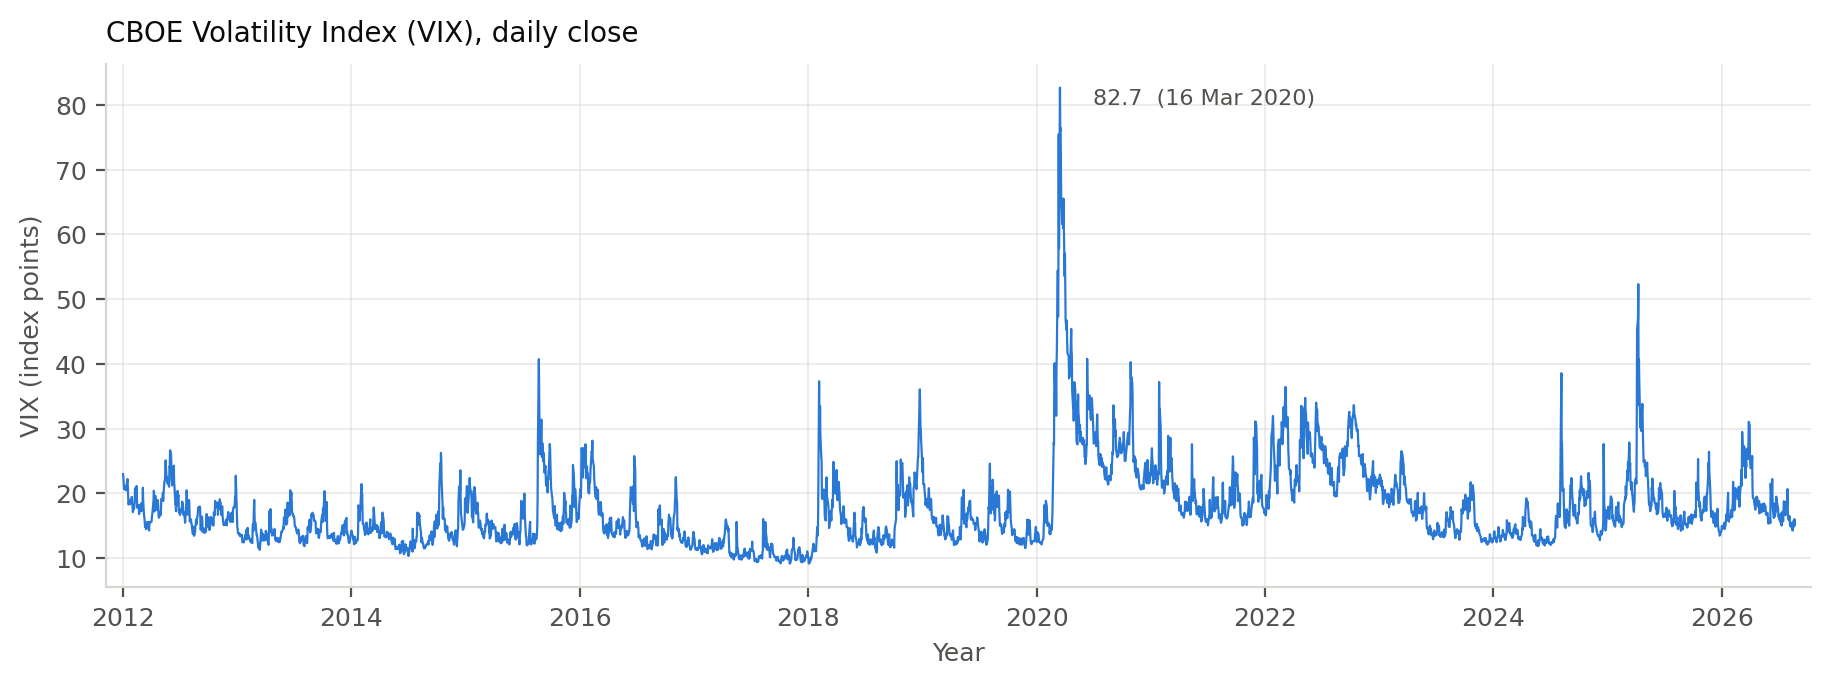
\includegraphics[width=\textwidth]{fig1_vix.png}
\caption{VIX, daily close, 2012--2026. Source: CBOE.}\label{fig:vix}
\end{figure}

\begin{figure}[H]\centering
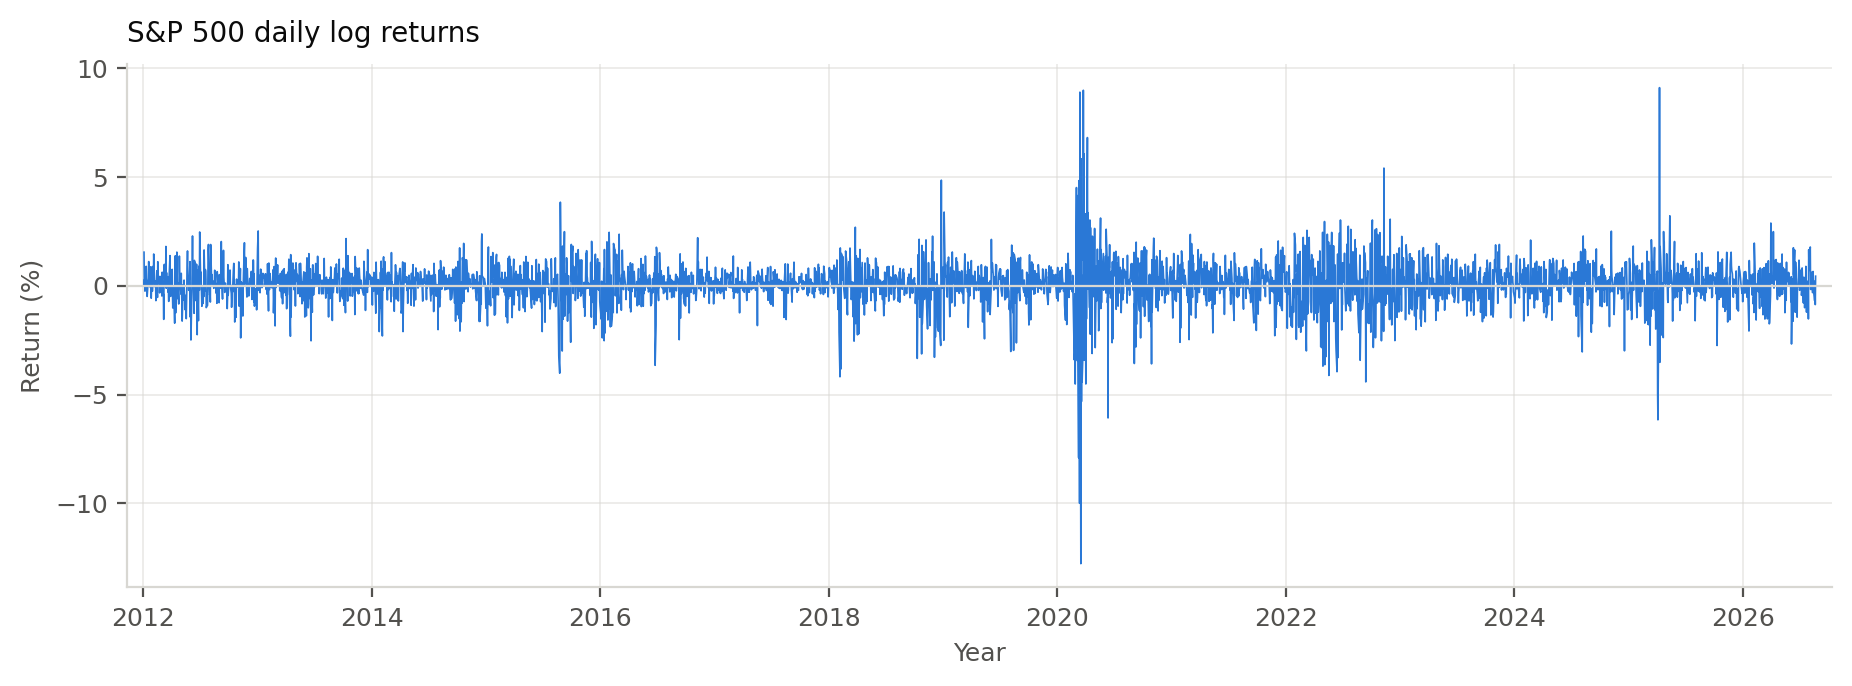
\includegraphics[width=\textwidth]{fig2_returns.png}
\caption{S\&P 500 daily log returns. Amplitude varies systematically over time.}
\label{fig:ret}
\end{figure}

\begin{figure}[H]\centering
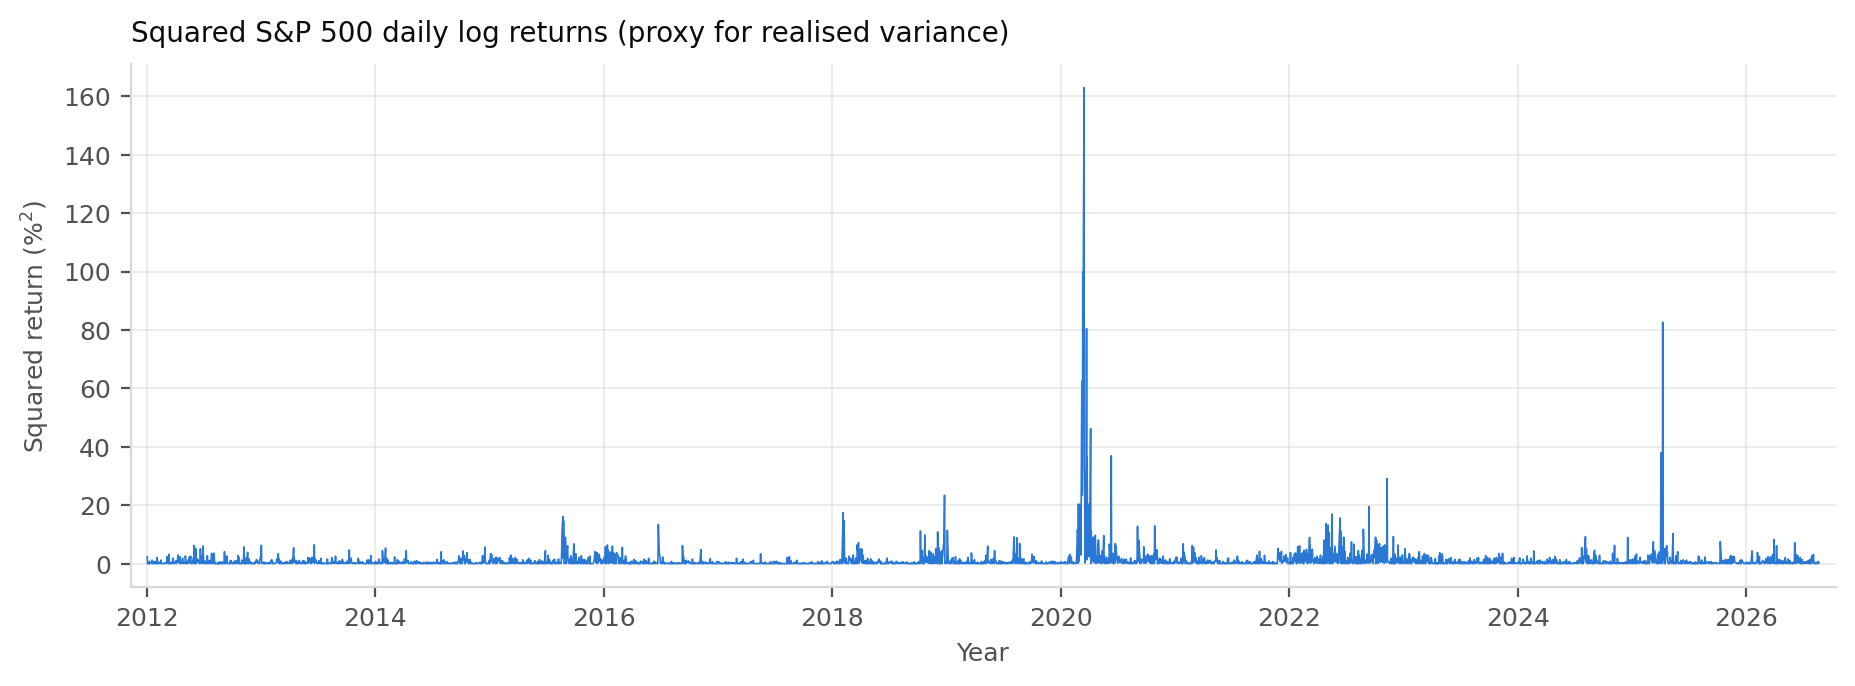
\includegraphics[width=\textwidth]{fig3_squared_returns.png}
\caption{Squared S\&P 500 daily log returns. Removing the sign makes the clustering of
large moves unmistakable.}\label{fig:sq}
\end{figure}

\begin{figure}[H]\centering
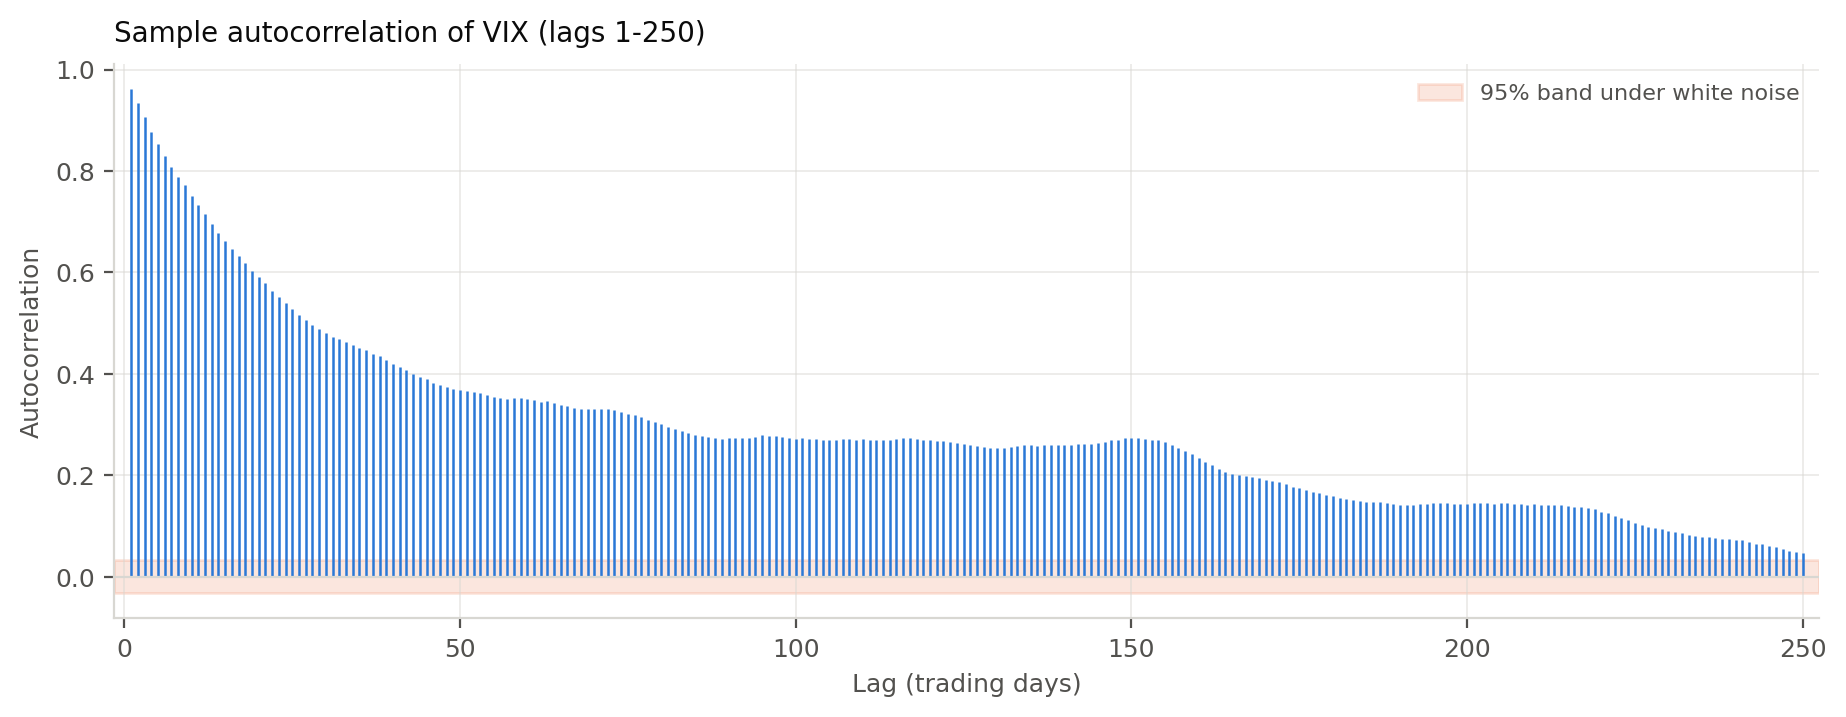
\includegraphics[width=\textwidth]{fig4_acf_vix.png}
\caption{Sample autocorrelation of VIX to lag 250. The ACF remains outside the 95\%
white-noise band across the entire range.}\label{fig:acfvix}
\end{figure}

\begin{figure}[H]\centering
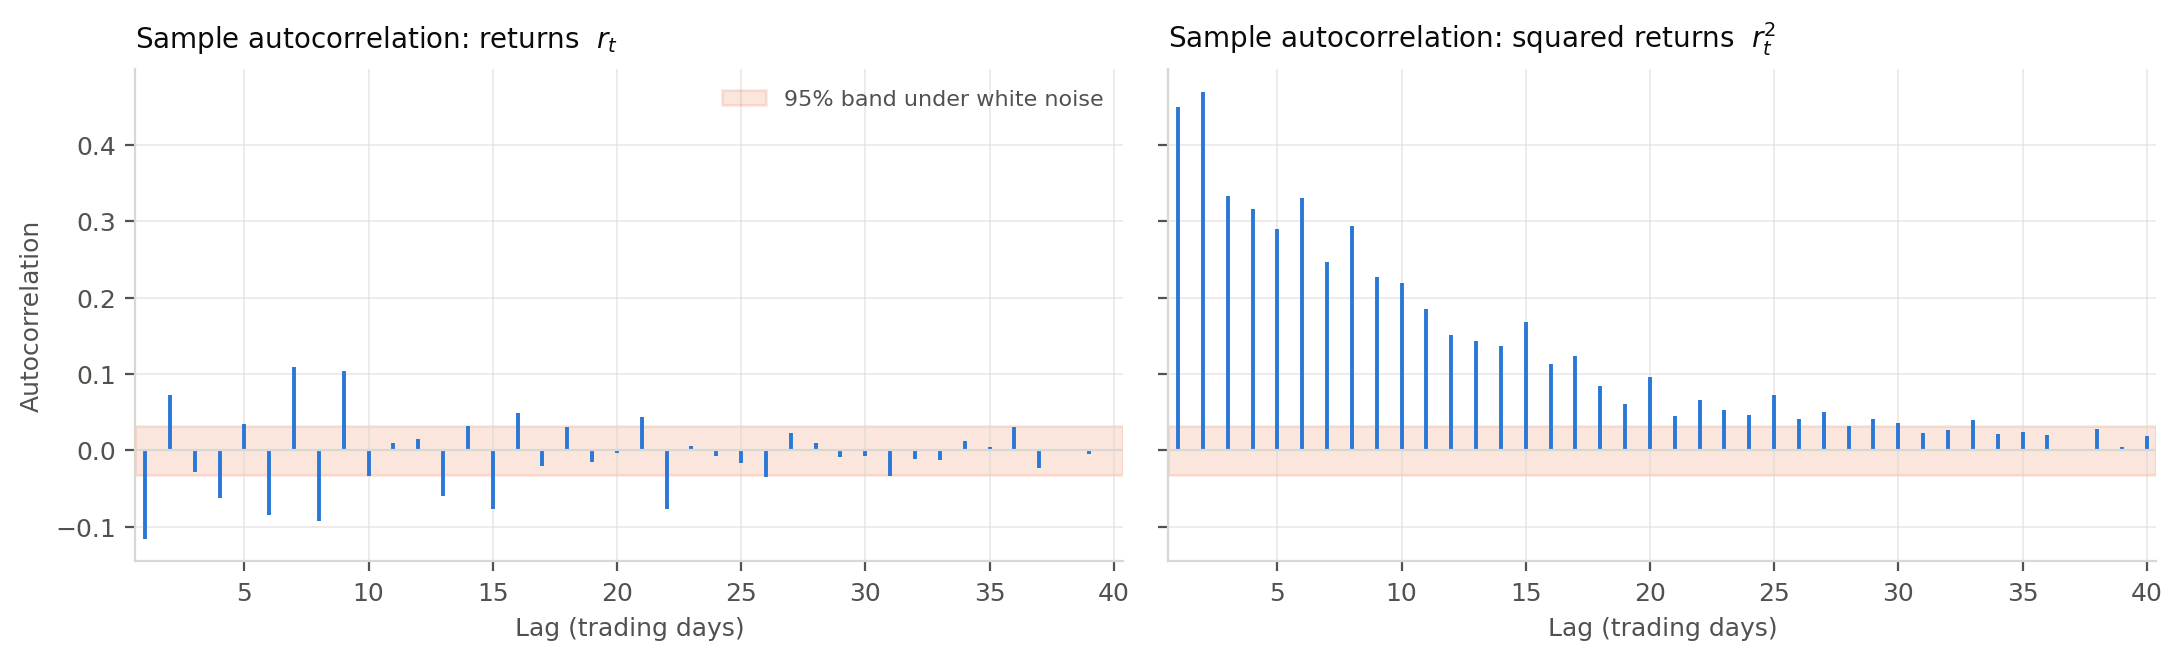
\includegraphics[width=\textwidth]{fig5_acf_returns.png}
\caption{Sample autocorrelation of returns (left) and squared returns (right). Direction
is unforecastable; magnitude is not.}\label{fig:acfret}
\end{figure}

\begin{figure}[H]\centering
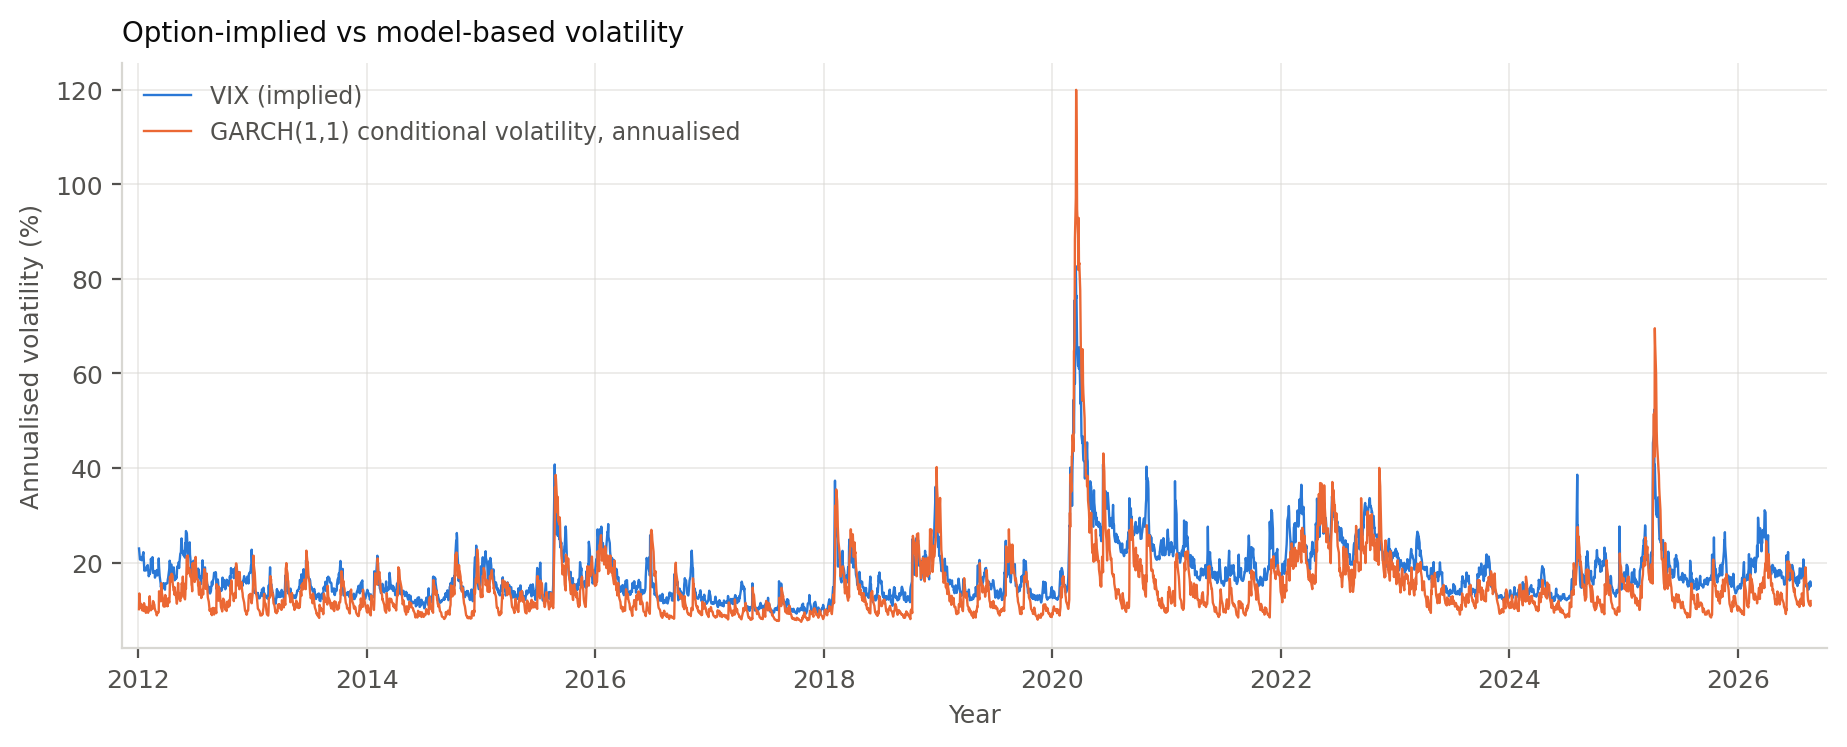
\includegraphics[width=\textwidth]{fig6_vix_vs_garch.png}
\caption{VIX against annualised GARCH(1,1) conditional volatility. Both series are in
annualised volatility points and share a single axis.}\label{fig:overlay}
\end{figure}

\begin{figure}[H]\centering
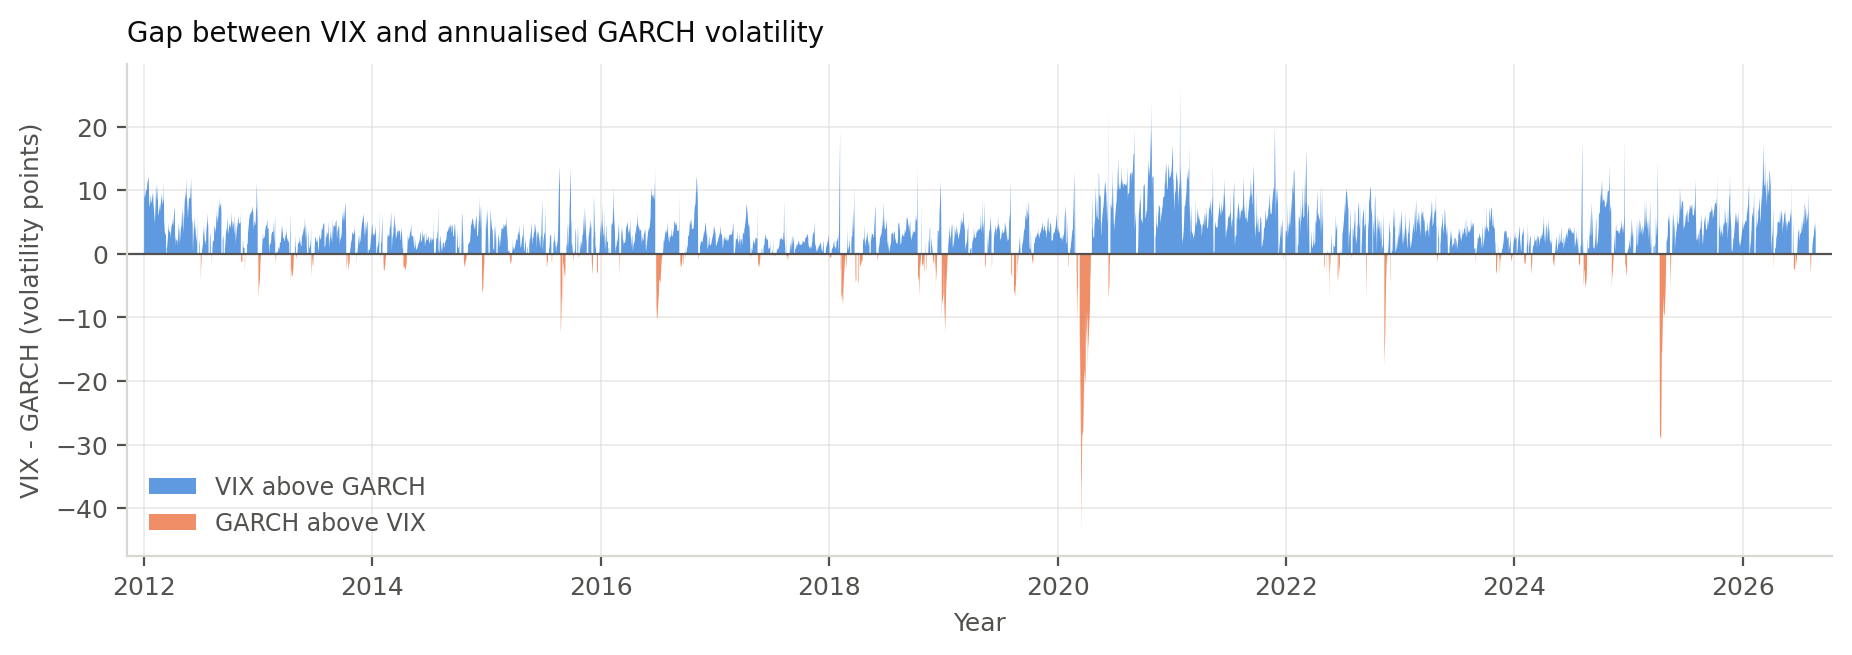
\includegraphics[width=\textwidth]{fig7_gap.png}
\caption{VIX minus annualised GARCH volatility. The predominance of positive values is
the variance risk premium; the negative spikes follow extreme single-day returns.}
\label{fig:gap}
\end{figure}

\end{document}
